\section{Jan Kusa}
\label{sec:jankusa}

I added a photo of a Chihuahua (see Figure~\ref{fig:dog}).

\begin{figure}[htbp] % Co oznacza [htbp]?
    \centering
    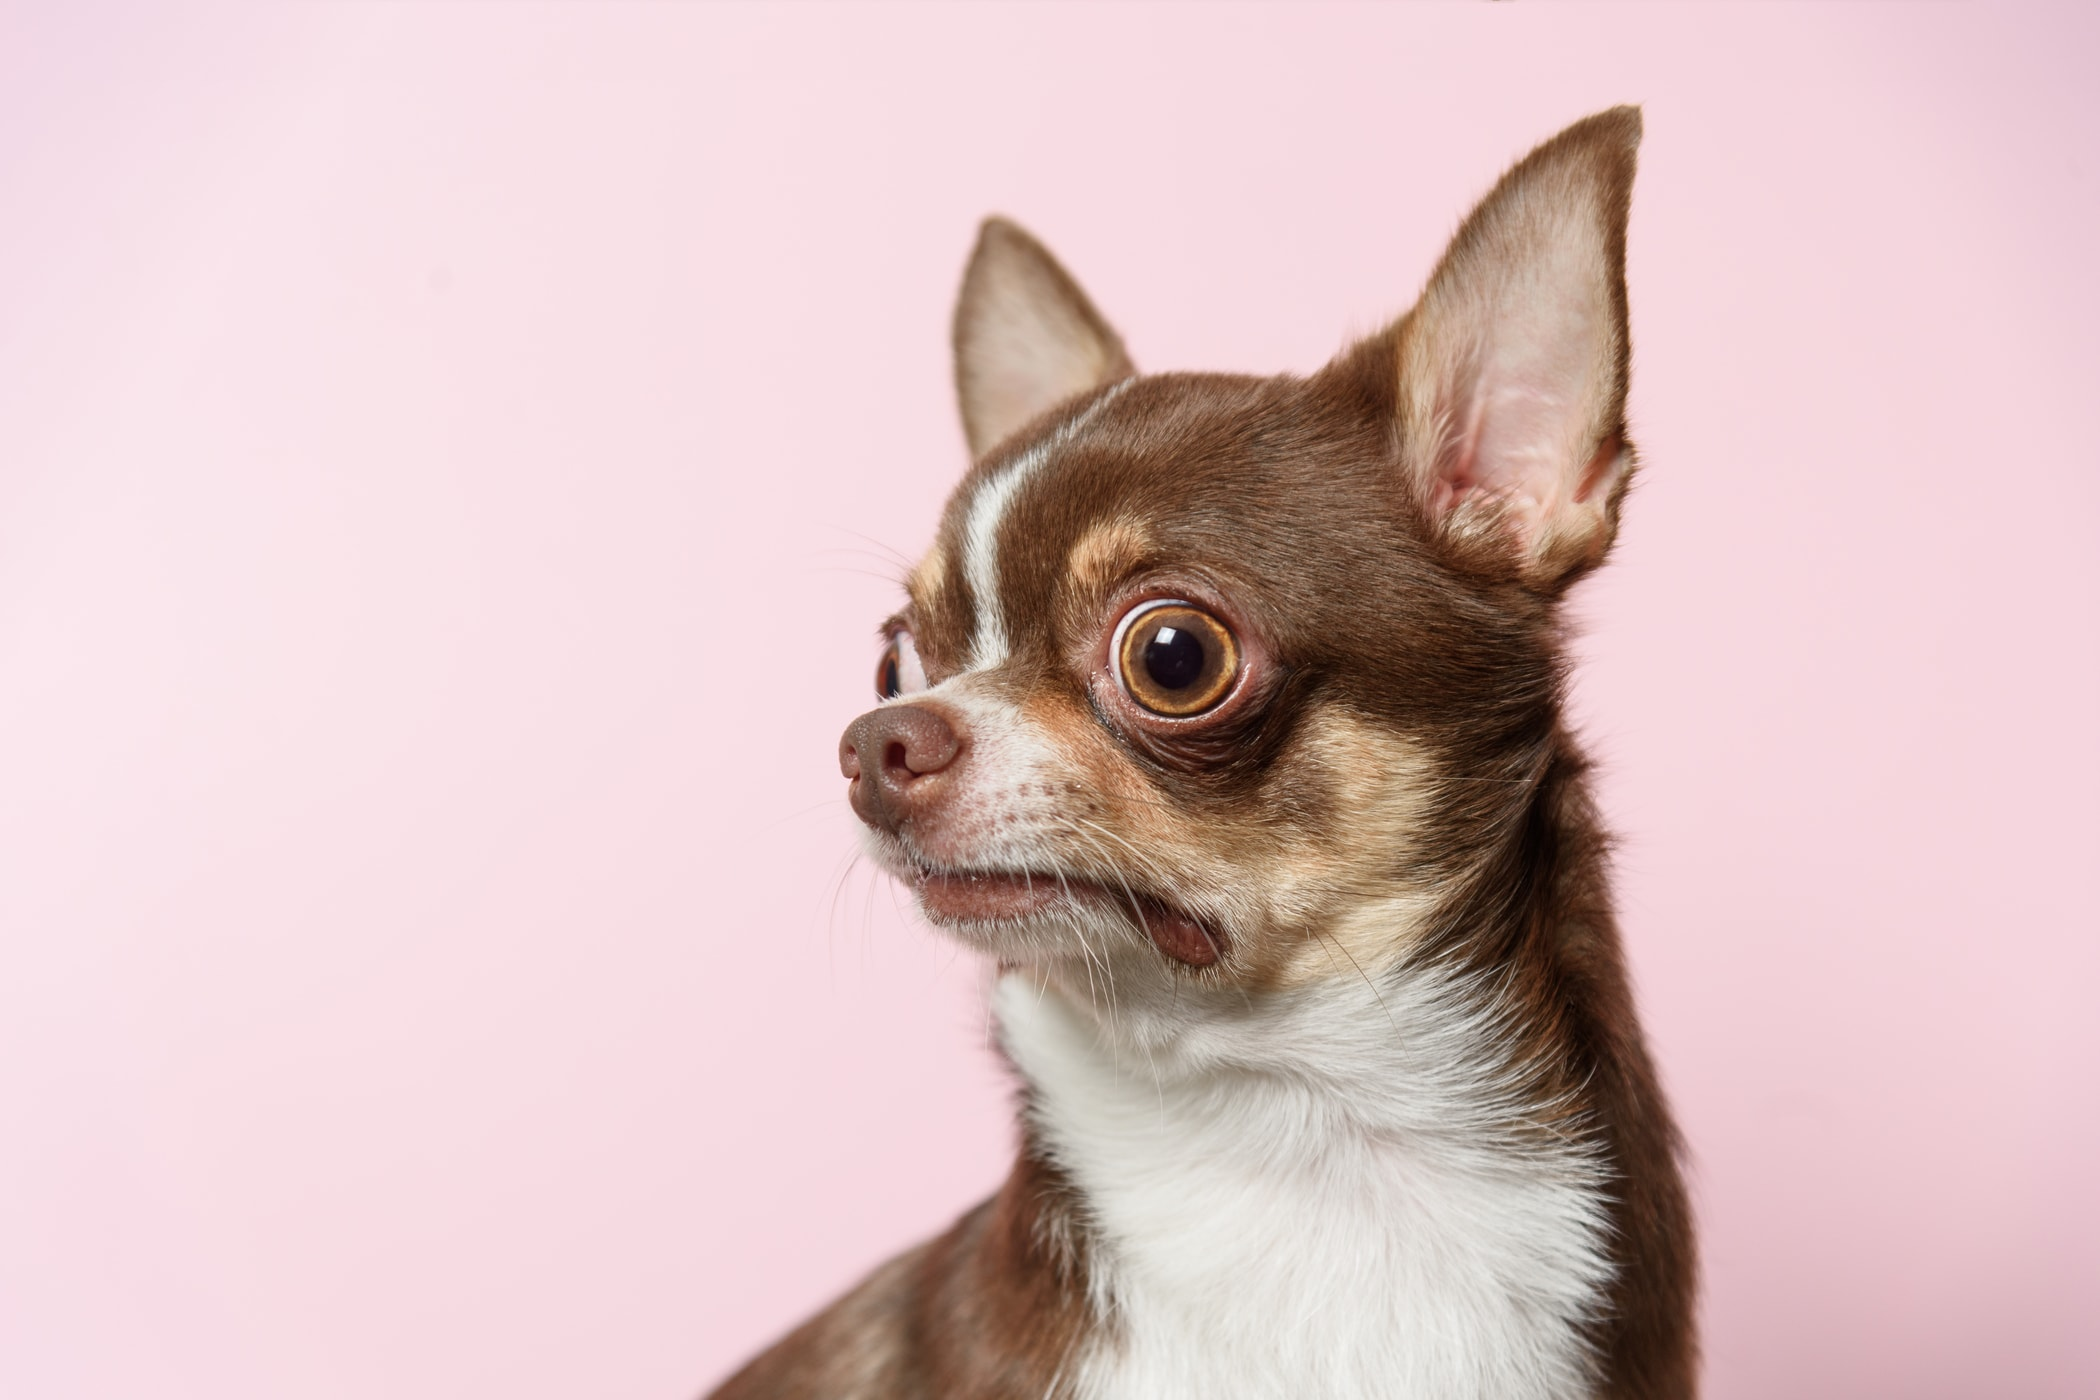
\includegraphics[width=0.5\textwidth]{pictures/chihuahua.jpg}
    \caption{This chihuahua is chic.}
    \label{fig:dog}
\end{figure}

\hline \hspace{1cm}\\

\textbf{Owoce:}
\begin{itemize}
  \item Jabłko
  \item Gruszka
  \item Banan
\end{itemize}

\textbf{Państwa o najwięszej powierzchni:}
\begin{enumerate}
  \item Rosja
  \item Kanada
  \item Chiny
\end{enumerate}

\hline \hspace{1cm}\\

\textbf{Tabela~\ref{tab:janek} prezentuje gre w "państwa-miasta".}


\begin{table}[htbp]
\begin{tabular}{|c|c|c|c|c|c|c|}
\hline
Litera & Państwo    & Miasto    & Zwierzę  & Roślina & Imię   & Punkty \\ \hline
A      & Albania    & Andrychów & Antylopa & Agrest  & Ania   & 45     \\ \hline
S      & Szwajcaria & Sewilla   & Słoń     & -       & Szymon & 35     \\ \hline
O      & Oman       & Oslo      & -        & Oliwka  & Olaf   & 40     \\ \hline
\end{tabular}
\caption{państwa-miasta}
\label{tab:janek}
\end{table}
\hline \hspace{1cm}\\

\textbf{Here is an interesting equation:}

\[z^n = r^n(cosnx + isinnx)\]

\newpage
\textbf{Chihuahua} - rasa psa należąca według klasyfikacji FCI do grupy psów ozdobnych i do towarzystwa, zaklasyfikowana do sekcji chihuahua, nie podlegająca próbom pracy. Istnieją dwie odmiany tej rasy: \textcolor{olive}{krótkowłosa} i \textcolor{blue}{długowłosa}. Zgodnie z klasyfikacją amerykańską, rasa ta należy do grupy psów ozdobnych i do towarzystwa. Typ wilkowaty.\par
\textbf{Rasy psa} - dawniej rasy (w znaczeniu zootechnicznym) zwierząt z gatunku psa domowego (\textit{Canis familiaris}) wyselekcjonowane głównie pod kątem wartości użytkowej, a współcześnie grupy psów uznanych przez organizację kynologiczną za spełniające wymogi wzorca rasy, ukierunkowanego głównie pod kątem wyglądu zewnętrznego, przekazujące swoje cechy fizyczne i psychiczne potomstwu. Różne stowarzyszenia kynologiczne stosują różne kryteria podziału tego gatunku na rasy oraz – zachowując odrębność w jeszcze większym stopniu – grupują rasy według swoich zasad, określonych we wzorcu rasy.